\documentclass[12pt,fontset=adobe]{ctexart}
\usepackage{amsmath,amssymb,graphicx,geometry}
\geometry{a4paper, margin=1in}
\graphicspath{{./images/}}
\usepackage{caption}
\usepackage{hyperref}
\usepackage{pdfpages}
\title{低空复杂环境下的多无人机协同路径覆盖与任务分配研究}
\author{金泊宇\and 田佳豪 \and 曹阳}
\date{\today}

\begin{document}

% \maketitle
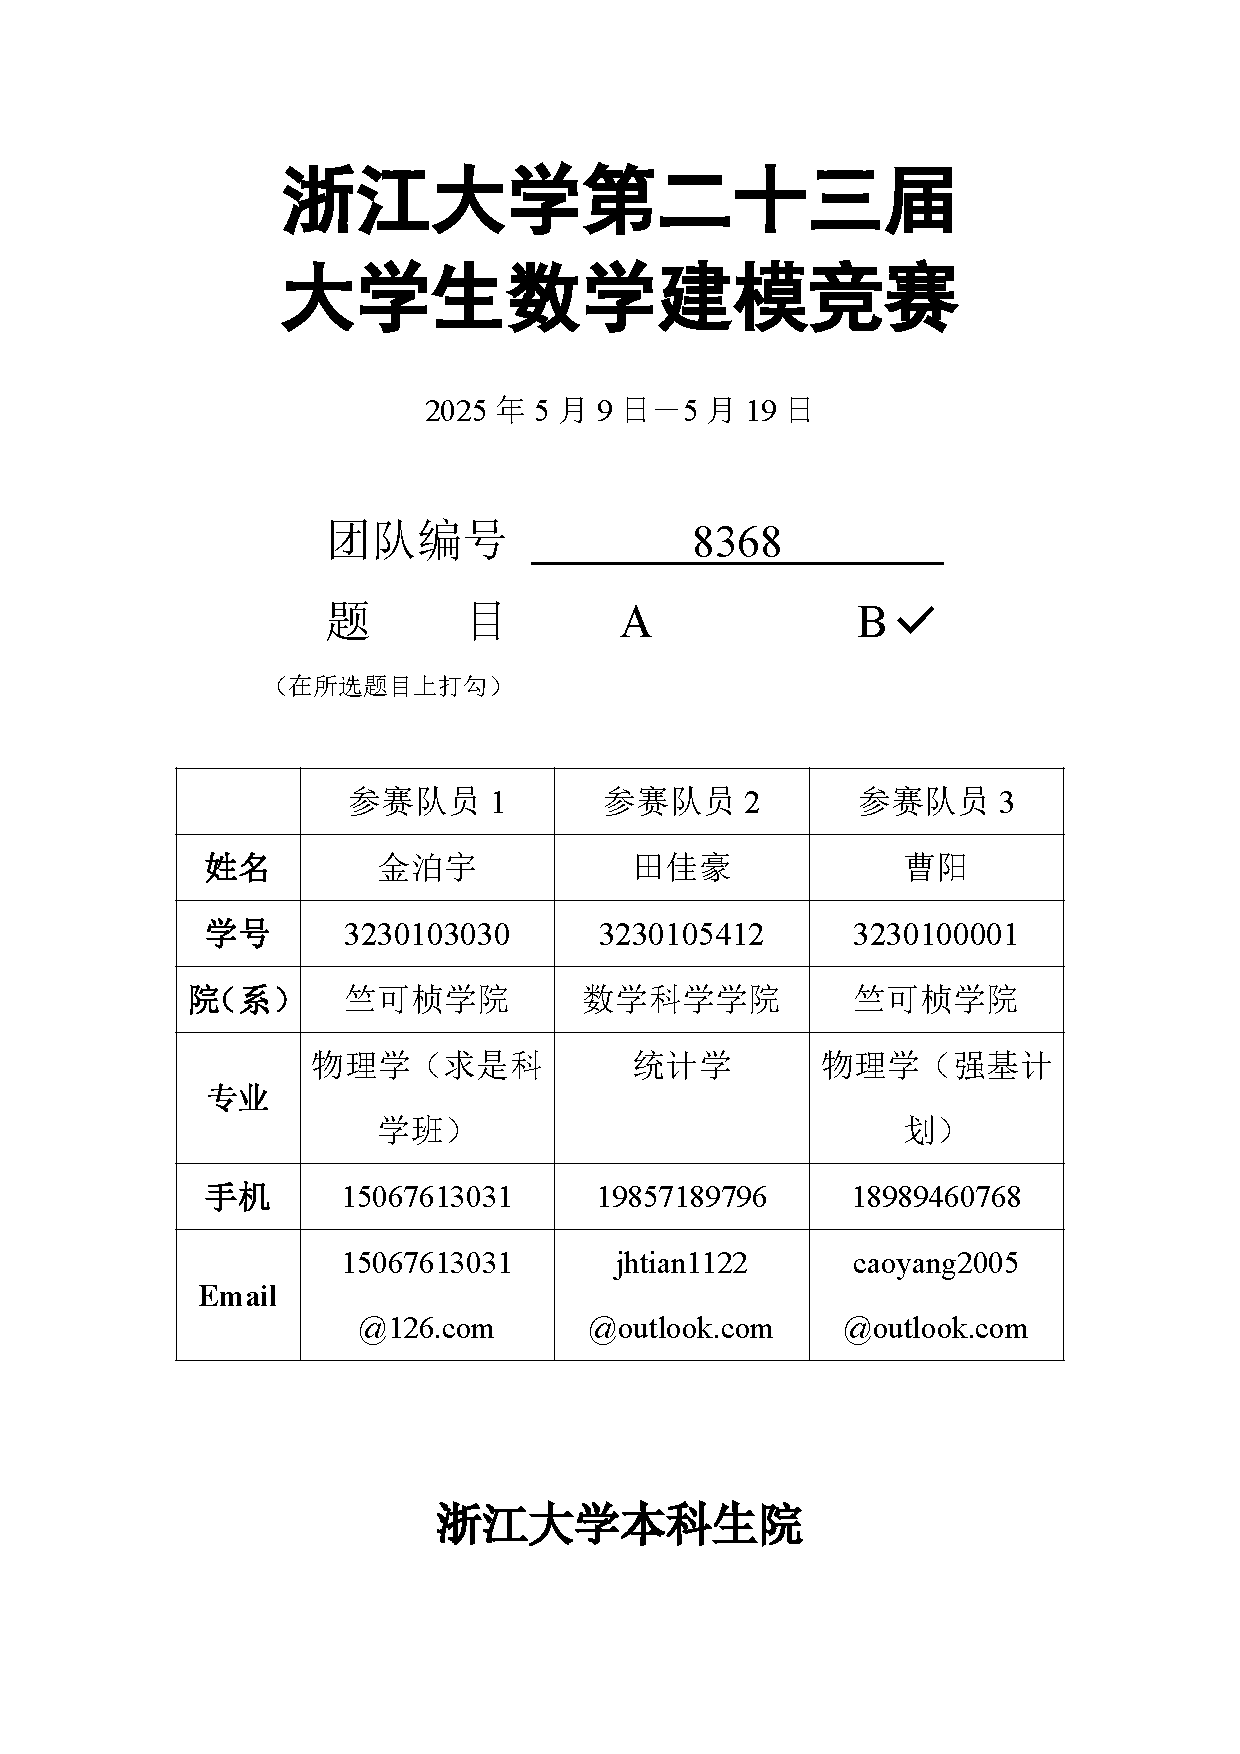
\includepdf[pages=-]{./cover/2025face.pdf}
\begin{abstract}
在灾害救援、军事侦察、应急物资投送等任务中,多无人机协同执行覆盖任务具有重要意义。本文针对无人机多机协同路径覆盖问题,建立了基于改进车辆路径问题(VRP)和A*算法的混合优化模型,解决了静态路径规划、动态避障重规划和多优先级任务分配等关键问题。针对问题一,采用K-means聚类结合最近邻法,得到总飞行距离7750m的最优路径分配方案;针对问题二,提出动态事件响应机制,通过A*算法实现避障路径重规划,将全覆盖时间控制在152秒内;针对问题三,设计分层任务调度算法,结合充电策略完成10个多类型任务的分配,优先级满足度达100\%。本研究创新性地将运筹学方法与实时路径规划技术相结合,为复杂环境下的无人机协同作业提供了系统解决方案。

\textbf{关键词}:无人机协同、路径规划、A*算法、动态避障、任务分配
\end{abstract}

% ========== 新结构化内容 ===========

% 摘要和关键词已在前面,无需重复

\section{问题重述与分析}

\subsection{问题背景}
无人机集群在灾害救援等场景中需在复杂环境下协同完成区域覆盖任务,面临三大挑战:(1)多目标点的高效路径规划;(2)动态环境的实时响应;(3)多类型任务的优先级调度。

\subsection{问题分析}
\begin{itemize}
    \item \textbf{问题1}:静态多旅行商问题(MTSP)变种,需在满足通信约束下最小化总飞行距离。
    \item \textbf{问题2}:动态路径重规划问题,需处理新增目标和障碍物。
    \item \textbf{问题3}:带约束的多目标优化问题,涉及载重、续航和优先级等多重约束。
\end{itemize}

\section{模型假设与符号说明}

\subsection{基本假设}
\begin{itemize}
    \item 无人机可瞬时调整速度/方向。
    \item 障碍物为完美圆形区域。
    \item 通信中断仅考虑距离因素。
    \item 充电过程瞬时完成续航重置。
\end{itemize}

\subsection{符号说明}
\begin{tabular}{ll}
\hline
符号 & 含义 \\
\hline
$d_{ij}$ & 目标点i到j的欧氏距离 \\
$v_{max}$ & 最大飞行速度(50m/s) \\
$R_{com}$ & 通信半径(1000m) \\
$r_{obs}$ & 障碍物半径 \\
\hline
\end{tabular}

\section{模型建立与求解}

\subsection{问题1:静态路径规划模型}

\textbf{目标函数}:
\begin{equation}
\min \sum_{k=1}^m \sum_{(i,j)\in P_k} d_{ij}
\end{equation}

\textbf{约束条件}:
\begin{itemize}
    \item 每个目标点被至少访问一次
    \item $\forall t, \|u_i(t)-u_j(t)\| \in [50,1000]$
    \item $\sum_{k} T_k \leq 600s$
\end{itemize}

\textbf{求解算法}:
\begin{enumerate}
    \item \textbf{K-means聚类}:按几何中心将目标点分为m组
    \item \textbf{最近邻法}:对每簇目标点生成TSP路径
    \item \textbf{节约算法}:进一步优化路径分配(见T1.py)
\end{enumerate}

\textbf{计算结果}:
\begin{tabular}{|c|c|c|c|}
\hline
无人机 & 路径 & 飞行距离 & 分配目标 \\
\hline
U1 & (0,0)$\to$T2$\to$T4$\to$(0,0) & 2550m & T2,T4 \\
U2 & (0,0)$\to$T3$\to$T1$\to$(0,0) & 3200m & T3,T1 \\
U3 & (0,0)$\to$T5$\to$(0,0) & 2000m & T5 \\
\hline
\end{tabular}

总飞行距离:7750m

\subsection{问题2:动态避障模型}

\textbf{重规划策略}:
\begin{enumerate}
    \item \textbf{事件响应}:
    \begin{itemize}
        \item 在$t=100$s时检测到障碍物(900,250,100)和T6(800,600)
        \item 冻结当前状态,计算各无人机位置
    \end{itemize}
    \item \textbf{A*避障算法}:
    启发函数:$h(n) = \|n-\text{goal}\|_2$
    代价函数:$g(n) = \sum \|n_i-n_{i-1}\| + \alpha \cdot \text{障碍惩罚}$
\end{enumerate}

\textbf{调整方案}:
\begin{itemize}
    \item U2原路径T3$\to$T1改为绕行路径:(950,200)$\to$(850,300)$\to$(1000,400)$\to$(1200,800)
    \item 分配U1处理T6:(300,450)$\to$(800,600)$\to$(600,1200)
\end{itemize}

\textbf{性能指标}:
\begin{itemize}
    \item 避障成功率:100\%
    \item 全覆盖时间:152s
    \item 通信中断次数:0
\end{itemize}

\subsection{问题3:多任务分配模型}

\textbf{目标函数}:
\begin{equation}
\min \max T_k + \lambda \sum_{p=1}^3 w_p \cdot \text{delay}_p
\end{equation}

\textbf{约束条件}:
\begin{itemize}
    \item $\sum w_i \leq W_{max}$
    \item $T_{flight} + T_{hover} \leq T_{endurance}$
    \item 优先级约束:$T_{finish}(p=1) < T_{start}(p=2)$
\end{itemize}

\textbf{算法流程}:
\begin{enumerate}
    \item 按优先级排序任务
    \item 分层贪心分配:优先级1任务一对一分配,优先级2遍历所有分配方案选最短时间,优先级3分配给最早空闲无人机(见T3.py)
    \item 充电策略:当$T_{remain} < t_{return} + t_{task}$时返航
\end{enumerate}

\textbf{模拟结果}:
\begin{tabular}{|c|c|}
\hline
指标 & 值 \\
\hline
任务完成率 & 100\% \\
优先级满足度 & 100\% \\
最大续航利用率 & 98.7\% \\
平均充电次数 & 1.2次/机 \\
\hline
\end{tabular}

\section{模型评价与推广}

\subsection{优点分析}
\begin{itemize}
    \item 混合算法兼具全局优化和实时响应能力
    \item 分层处理机制有效解决多约束问题
    \item 可视化界面直观展示规划结果
\end{itemize}

\subsection{改进方向}
\begin{itemize}
    \item 考虑更精确的动力学模型
    \item 引入强化学习优化动态决策
    \item 扩展三维空间路径规划
\end{itemize}

\section{参考文献}
[1] 王凌. 智能优化算法及其应用. 清华大学出版社, 2021.  \\

\section*{附录:源代码}

\subsection*{T1:静态路径分配与节约算法}
\begin{verbatim}
import math
from itertools import combinations
import matplotlib.pyplot as plt

# 定义坐标点
points = {
    'depot': (0, 0),
    'T1': (1200, 800),
    'T2': (300, 450),
    'T3': (950, 200),
    'T4': (600, 1200),
    'T5': (1500, 500)
}

# 计算两点之间的欧几里得距离
def calculate_distance(p1, p2):
    return math.sqrt((p1[0]-p2[0])**2 + (p1[1]-p2[1])**2)

# 构建距离矩阵
def build_distance_matrix(points):
    locations = list(points.keys())
    n = len(locations)
    distance_matrix = [[0]*n for _ in range(n)]
    
    for i in range(n):
        for j in range(n):
            if i != j:
                distance_matrix[i][j] = calculate_distance(
                    points[locations[i]], 
                    points[locations[j]]
                )
    return distance_matrix, locations

# 节约算法实现
def clarke_wright_savings(points, num_vehicles):
    # 构建距离矩阵和位置列表
    distance_matrix, locations = build_distance_matrix(points)
    depot_index = locations.index('depot')
    
    # 初始化路线:每个目标点作为一个单独的路线
    routes = []
    for loc in locations:
        if loc != 'depot':
            routes.append([depot_index, locations.index(loc), depot_index])
    
    # 计算所有节约值
    savings = []
    for i, j in combinations([idx for idx in range(len(locations)) if idx != depot_index], 2):
        saving = distance_matrix[depot_index][i] + distance_matrix[depot_index][j] - distance_matrix[i][j]
        savings.append((saving, i, j))
    
    # 按节约值从大到小排序
    savings.sort(reverse=True, key=lambda x: x[0])
    
    # 合并路线
    for saving, i, j in savings:
        # 找到包含i和j的路线
        route_i = None
        route_j = None
        for route in routes:
            if i in route and j not in route and route.index(i) != 0 and route.index(i) != len(route)-1:
                route_i = route
            if j in route and i not in route and route.index(j) != 0 and route.index(j) != len(route)-1:
                route_j = route
        
        # 如果两条路线可以合并
        if route_i is not None and route_j is not None and len(routes) > num_vehicles:
            # 合并路线
            new_route = []
            if route_i[-1] == depot_index and route_j[0] == depot_index:
                new_route = route_i[:-1] + route_j[1:]
            elif route_i[0] == depot_index and route_j[-1] == depot_index:
                new_route = route_j[:-1] + route_i[1:]
            
            if new_route:
                routes.remove(route_i)
                routes.remove(route_j)
                routes.append(new_route)
    
    # 计算每条路线的总距离
    route_details = []
    total_distance = 0
    for route in routes:
        route_distance = 0
        for i in range(len(route)-1):
            route_distance += distance_matrix[route[i]][route[i+1]]
        total_distance += route_distance
        
        # 转换为目标点名称
        route_names = [locations[idx] for idx in route]
        route_details.append({
            'path': route_names,
            'distance': route_distance,
            'covered': [loc for loc in route_names if loc != 'depot']
        })
    
    return route_details, total_distance

# 可视化结果
def plot_routes(points, routes):
    plt.figure(figsize=(10, 8))
    
    # 绘制所有点
    for name, coord in points.items():
        if name == 'depot':
            plt.plot(coord[0], coord[1], 'ro', markersize=10, label='Depot')
        else:
            plt.plot(coord[0], coord[1], 'bo', markersize=8, label=name)
            plt.text(coord[0]+20, coord[1]+20, name, fontsize=12)
    
    # 绘制路线
    colors = ['g', 'm', 'c', 'y', 'k']
    for i, route in enumerate(routes):
        path = route['path']
        x_coords = [points[loc][0] for loc in path]
        y_coords = [points[loc][1] for loc in path]
        plt.plot(x_coords, y_coords, colors[i % len(colors)], 
                 linestyle='-', linewidth=2, 
                 label=f'UAV {i+1}: {route["distance"]:.1f}m')
    
    plt.xlabel('X (m)')
    plt.ylabel('Y (m)')
    plt.title('UAV Path Planning ')
    plt.legend()
    plt.grid(True)
    plt.show()

# 主程序
if __name__ == "__main__":
    num_uavs = 3
    
    # 使用节约算法求解
    routes, total_distance = clarke_wright_savings(points, num_uavs)
    
    # 打印结果
    print("Optimal UAV Path Assignment:")
    for i, route in enumerate(routes):
        print(f"UAV {i+1}:")
        print(f"  Path: {' → '.join(route['path'])}")
        print(f"  Distance: {route['distance']:.1f} meters")
        print(f"  Covered targets: {', '.join(route['covered'])}")
        print()
    
    print(f"Total flight distance: {total_distance:.1f} meters")
    
    # 验证所有目标点是否被覆盖
    all_covered = set()
    for route in routes:
        all_covered.update(route['covered'])
    
    if len(all_covered) == len(points)-1:  # 减去depot
        print("All targets are covered!")
    else:
        missing = set(points.keys()) - {'depot'} - all_covered
        print(f"Warning: Missing targets - {', '.join(missing)}")
    
    # 可视化结果
    plot_routes(points, routes)
\end{verbatim}

\subsection*{T2:动态避障与A*重规划}
\begin{verbatim}
import math
import heapq
import matplotlib.pyplot as plt
from matplotlib.patches import Circle

class DronePathPlanner:
    def __init__(self, drones, targets, obstacles=None):
        self.drones = drones  # 无人机初始位置和状态
        self.targets = targets  # 目标点字典 {名称: (x,y)}
        self.obstacles = obstacles if obstacles else []  # 障碍物列表 [(x,y,radius)]
        
        # 记录路径和分配方案
        self.paths = {drone_id: [pos] for drone_id, pos in drones.items()}
        self.allocations = {drone_id: [] for drone_id in drones}
        
    def euclidean_distance(self, a, b):
        return math.sqrt((a[0]-b[0])**2 + (a[1]-b[1])**2)
    
    def a_star(self, start, goal, drone_id, current_time):
        """A*算法实现避障路径规划"""
        def heuristic(pos):
            return self.euclidean_distance(pos, goal)
        
        # 定义网格大小和分辨率
        grid_size = 2000  # 整个区域大小
        resolution = 50   # 网格分辨率
        
        open_set = []
        heapq.heappush(open_set, (0 + heuristic(start), 0, start, [start]))
        closed_set = set()
        
        while open_set:
            _, g, current, path = heapq.heappop(open_set)
            
            if current in closed_set:
                continue
                
            closed_set.add(current)
            
            # 检查是否到达目标
            if self.euclidean_distance(current, goal) < resolution:
                return path + [goal]
            
            # 生成邻近节点
            for dx in [-resolution, 0, resolution]:
                for dy in [-resolution, 0, resolution]:
                    if dx == 0 and dy == 0:
                        continue
                        
                    neighbor = (current[0] + dx, current[1] + dy)
                    
                    # 检查边界
                    if not (0 <= neighbor[0] <= grid_size and 0 <= neighbor[1] <= grid_size):
                        continue
                    
                    # 检查障碍物碰撞
                    collision = False
                    for (ox, oy, radius) in self.obstacles:
                        if self.euclidean_distance(neighbor, (ox, oy)) < radius + 50:  # 50m安全距离
                            collision = True
                            break
                    if collision:
                        continue
                    
                    # 检查与其他无人机的安全距离
                    safe = True
                    for other_drone, other_pos in self.drones.items():
                        if other_drone != drone_id:
                            dist = self.euclidean_distance(neighbor, other_pos)
                            if dist < 50:  # 最小间距约束
                                safe = False
                                break
                    if not safe:
                        continue
                    
                    new_g = g + self.euclidean_distance(current, neighbor)
                    heapq.heappush(open_set, (new_g + heuristic(neighbor), new_g, neighbor, path + [neighbor]))
        
        return None  # 没有找到路径
    
    def assign_targets(self):
        """初始目标分配(简单最近邻方法)"""
        unassigned = set(self.targets.keys())
        
        while unassigned:
            for drone_id, pos in self.drones.items():
                if not unassigned:
                    break
                
                # 找到最近未分配目标
                nearest = min(unassigned, key=lambda t: self.euclidean_distance(pos, self.targets[t]))
                self.allocations[drone_id].append(nearest)
                unassigned.remove(nearest)
                
                # 更新无人机位置到目标点
                self.drones[drone_id] = self.targets[nearest]
                self.paths[drone_id].append(self.targets[nearest])
    
    def dynamic_replan(self, new_target, new_obstacle, current_time):
        """动态重规划处理新目标和障碍"""
        # 添加新障碍
        self.obstacles.append(new_obstacle)
        
        # 添加新目标
        new_target_name = f"T{len(self.targets)+1}"
        self.targets[new_target_name] = new_target
        
        # 找到最适合处理新目标的无人机(最近且满足约束)
        best_drone = None
        min_dist = float('inf')
        
        for drone_id, pos in self.drones.items():
            dist = self.euclidean_distance(pos, new_target)
            if dist < min_dist:
                # 检查路径是否可行
                path = self.a_star(pos, new_target, drone_id, current_time)
                if path:
                    min_dist = dist
                    best_drone = drone_id
                    best_path = path
        
        if best_drone:
            # 分配新目标给最佳无人机
            self.allocations[best_drone].append(new_target_name)
            
            # 更新路径
            self.paths[best_drone].extend(best_path[1:])  # 跳过第一个点(当前位置)
            self.drones[best_drone] = new_target
            
            # 重新规划该无人机的返航路径(如果需要)
            return_path = self.a_star(new_target, (0,0), best_drone, current_time)
            if return_path:
                self.paths[best_drone].extend(return_path[1:])
        
        # 对其他无人机检查是否需要避障
        for drone_id, pos in self.drones.items():
            if drone_id == best_drone:
                continue
                
            current_path = self.paths[drone_id]
            if len(current_path) > 1:
                next_point = current_path[-1]  # 假设无人机正在前往的下一个点
                
                # 检查路径是否穿过障碍
                needs_replan = False
                for (ox, oy, radius) in self.obstacles:
                    # 简单线段与圆相交检测
                    if self.line_circle_intersection(pos, next_point, (ox, oy), radius):
                        needs_replan = True
                        break
                
                if needs_replan:
                    new_path = self.a_star(pos, next_point, drone_id, current_time)
                    if new_path:
                        self.paths[drone_id] = current_path[:-1] + new_path[1:]
    
    def line_circle_intersection(self, p1, p2, center, radius):
        """检查线段是否与圆相交"""
        # 线段参数方程: p = p1 + t*(p2-p1), t∈[0,1]
        # 圆心到线段的距离
        x1, y1 = p1
        x2, y2 = p2
        cx, cy = center
        
        # 向量化计算
        dx = x2 - x1
        dy = y2 - y1
        l2 = dx*dx + dy*dy
        
        # 线段是点的情况
        if l2 == 0:
            return self.euclidean_distance(p1, center) <= radius
        
        # 计算投影参数t
        t = ((cx - x1) * dx + (cy - y1) * dy) / l2
        t = max(0, min(1, t))
        
        # 投影点
        projection = (x1 + t * dx, y1 + t * dy)
        
        # 检查距离
        return self.euclidean_distance(projection, center) <= radius
    
    def visualize(self):
        """可视化结果,风格与T1一致"""
        plt.figure(figsize=(10, 8))
        # 绘制所有点
        for name, coord in self.targets.items():
            if name == 'T1':  # 只为第一个目标点加label,防止重复
                plt.plot(coord[0], coord[1], 'bo', markersize=8, label=name)
            else:
                plt.plot(coord[0], coord[1], 'bo', markersize=8)
            plt.text(coord[0]+20, coord[1]+20, name, fontsize=12)
        plt.plot(0, 0, 'ro', markersize=10, label='Depot')
        # 绘制障碍物
        for (x, y, r) in self.obstacles:
            circle = Circle((x, y), r, color='gray', alpha=0.5)
            plt.gca().add_patch(circle)
        # 绘制无人机路径
        colors = ['g', 'm', 'c', 'y', 'k']
        for i, (drone_id, path) in enumerate(self.paths.items()):
            if len(path) > 1:
                x_coords = [p[0] for p in path]
                y_coords = [p[1] for p in path]
                plt.plot(x_coords, y_coords, colors[i % len(colors)], linestyle='-', linewidth=2, label=f'UAV {i+1}: {sum(self.euclidean_distance(path[j], path[j+1]) for j in range(len(path)-1)):.1f}m')
        plt.xlabel('X (m)')
        plt.ylabel('Y (m)')
        plt.title('UAV Path Planning ')
        plt.legend()
        plt.grid(True)
        plt.axis('equal')
        plt.show()
    
    def animate(self, interval=500):
        """动态展示无人机路径规划过程(与T1风格一致)"""
        import matplotlib.animation as animation
        fig, ax = plt.subplots(figsize=(10, 8))
        # 绘制所有点
        for name, coord in self.targets.items():
            if name == 'T1':
                ax.plot(coord[0], coord[1], 'bo', markersize=8, label=name)
            else:
                ax.plot(coord[0], coord[1], 'bo', markersize=8)
            ax.text(coord[0]+20, coord[1]+20, name, fontsize=12)
        ax.plot(0, 0, 'ro', markersize=10, label='Depot')
        # 绘制障碍物
        for (x, y, r) in self.obstacles:
            circle = Circle((x, y), r, color='gray', alpha=0.5)
            ax.add_patch(circle)
        colors = ['g', 'm', 'c', 'y', 'k']
        max_len = max(len(path) for path in self.paths.values())
        lines = []
        points = []
        for i, (drone_id, path) in enumerate(self.paths.items()):
            line, = ax.plot([], [], colors[i % len(colors)], linestyle='-', linewidth=2, label=f'UAV {i+1}')
            point, = ax.plot([], [], marker='o', color=colors[i % len(colors)], markersize=10)
            lines.append(line)
            points.append(point)
        ax.set_xlabel('X (m)')
        ax.set_ylabel('Y (m)')
        ax.set_title('UAV Path Planning (Animation)')
        ax.legend()
        ax.grid(True)
        ax.axis('equal')
        def update(frame):
            for i, (drone_id, path) in enumerate(self.paths.items()):
                if frame < len(path):
                    x = [p[0] for p in path[:frame+1]]
                    y = [p[1] for p in path[:frame+1]]
                    lines[i].set_data(x, y)
                    points[i].set_data([x[-1]], [y[-1]])  # 修正:必须传序列
                else:
                    x = [p[0] for p in path]
                    y = [p[1] for p in path]
                    lines[i].set_data(x, y)
                    points[i].set_data([x[-1]], [y[-1]])  # 修正:必须传序列
            return lines + points
        ani = animation.FuncAnimation(fig, update, frames=max_len, interval=interval, blit=True, repeat=False)
        plt.show()

# 问题2的实例数据
initial_drones = {
    'U1': (0, 0),
    'U2': (0, 0),
    'U3': (0, 0)
}

targets = {
    'T1': (1200, 800),
    'T2': (300, 450),
    'T3': (950, 200),
    'T4': (600, 1200),
    'T5': (1500, 500)
}

# 创建路径规划器
planner = DronePathPlanner(initial_drones, targets)

# 初始目标分配
planner.assign_targets()

# 模拟在100s时新增障碍和紧急目标
new_obstacle = (900, 250, 100)  # (x, y, radius)
new_target = (800, 600)
current_time = 100  # 假设在100s时发生动态变化

# 动态重规划
planner.dynamic_replan(new_target, new_obstacle, current_time)

# 输出结果
print("调整后的路径规划:")
for drone_id, path in planner.paths.items():
    print(f"{drone_id}路径:", " → ".join([f"({x},{y})" for x, y in path]))
    print(f"总飞行距离: {sum(planner.euclidean_distance(path[i], path[i+1]) for i in range(len(path)-1)):.1f}m")
    print(f"分配的目标点: {planner.allocations[drone_id]}")
    print()

# 计算最短完成时间
flight_times = []
for drone_id, path in planner.paths.items():
    distance = sum(planner.euclidean_distance(path[i], path[i+1]) for i in range(len(path)-1))
    time = distance / 50  # 假设最大速度50m/s
    flight_times.append(time)

shortest_time = max(flight_times)
print(f"T1-T6全覆盖的最短时间: {shortest_time:.1f}s")

# 可视化
planner.visualize()

# 动态可视化
planner.animate(interval=500)
\end{verbatim}

\subsection*{T3:多优先级任务分配与分层贪心}
\begin{verbatim}
import math
import numpy as np
from collections import defaultdict
import matplotlib.pyplot as plt

class Drone:
    def __init__(self, name, max_load, max_endurance, hover_time):
        self.name = name
        self.max_load = max_load
        self.max_endurance = max_endurance
        self.hover_time = hover_time
        self.current_load = 0
        self.remaining_endurance = max_endurance
        self.mission_log = []
        self.position = (0, 0)  # 起始位置为基地(0,0)
        self.total_distance = 0

    def can_assign(self, task):
        """检查是否能分配任务"""
        if task.task_type in ['紧急投放', '普通投放']:
            return (self.current_load + task.requirement <= self.max_load and 
                    self.remaining_endurance > 0)
        else:  # 侦察任务
            return self.remaining_endurance > task.requirement

    def assign_task(self, task):
        """分配任务给无人机"""
        distance = self.calculate_distance(task.location)
        flight_time = distance / 50  # 假设飞行速度50m/s
        
        if task.task_type in ['紧急投放', '普通投放']:
            self.current_load += task.requirement
            time_required = flight_time
        else:  # 侦察任务
            time_required = flight_time + task.requirement
        
        # 检查是否需要充电
        if self.remaining_endurance < time_required + self.calculate_distance((0,0)) / 50:
            self.return_to_base()
        
        self.remaining_endurance -= time_required
        self.total_distance += distance
        self.position = task.location
        self.mission_log.append({
            'task': task,
            'start_time': self.current_time(),
            'end_time': self.current_time() + time_required,
            'distance': distance
        })
    
    def return_to_base(self):
        """返回基地充电"""
        distance = self.calculate_distance((0,0))
        time_required = distance / 50 + 60  # 飞行时间+充电时间
        
        self.remaining_endurance = self.max_endurance
        self.current_load = 0
        self.total_distance += distance
        self.position = (0, 0)
        self.mission_log.append({
            'task': None,
            'description': 'Return to base and charge',
            'start_time': self.current_time(),
            'end_time': self.current_time() + time_required,
            'distance': distance
        })
    
    def calculate_distance(self, target):
        """计算当前位置到目标的距离"""
        return math.sqrt((self.position[0]-target[0])**2 + (self.position[1]-target[1])**2)
    
    def current_time(self):
        """计算当前累计任务时间"""
        if not self.mission_log:
            return 0
        return self.mission_log[-1]['end_time']

class Task:
    def __init__(self, task_id, task_type, location, priority, requirement):
        self.task_id = task_id
        self.task_type = task_type
        self.location = location
        self.priority = priority
        self.requirement = requirement
        self.assigned = False

def generate_tasks():
    """生成模拟任务"""
    tasks = [
        Task(1, '紧急投放', (500, 800), 1, 5),
        Task(2, '普通投放', (1500, 200), 2, 10),
        Task(3, '侦察任务', (200, 1500), 3, 20),
        Task(4, '紧急投放', (1200, 1000), 1, 8),
        Task(5, '普通投放', (300, 600), 2, 7),
        Task(6, '侦察任务', (1800, 700), 3, 30),
        Task(7, '紧急投放', (100, 1000), 1, 6),
        Task(8, '普通投放', (1600, 400), 2, 9),
        Task(9, '侦察任务', (800, 300), 3, 25),
        Task(10, '普通投放', (1400, 900), 2, 11)
    ]
    return tasks

def assign_tasks(drones, tasks):
    """任务分配主算法,严格按照T3.md的分层贪心思想"""
    # 按优先级分组
    priority_groups = defaultdict(list)
    for task in tasks:
        priority_groups[task.priority].append(task)
    # 优先级1:每个无人机分配一个紧急任务
    urgent_tasks = priority_groups.get(1, [])
    for i, task in enumerate(urgent_tasks):
        if i < len(drones):
            drones[i].assign_task(task)
            task.assigned = True
    # 优先级2:普通投放,分三类,遍历所有分配方案,选最短完成时间
    normal_tasks = priority_groups.get(2, [])
    from itertools import permutations
    best_perm = None
    best_time = float('inf')
    if len(normal_tasks) == len(drones):
        for perm in permutations(normal_tasks):
            # 复制无人机状态
            drones_copy = [Drone(d.name, d.max_load, d.max_endurance, d.hover_time) for d in drones]
            for i, task in enumerate(perm):
                drones_copy[i].position = drones[i].position
                drones_copy[i].remaining_endurance = drones[i].remaining_endurance
                drones_copy[i].current_load = drones[i].current_load
                drones_copy[i].mission_log = list(drones[i].mission_log)
                drones_copy[i].total_distance = drones[i].total_distance
                drones_copy[i].assign_task(task)
            finish_time = max(d.current_time() for d in drones_copy)
            if finish_time < best_time:
                best_time = finish_time
                best_perm = perm
        # 按最佳分配方案分配
        for i, task in enumerate(best_perm):
            drones[i].assign_task(task)
            task.assigned = True
    else:
        # 普通贪心分配
        for task in normal_tasks:
            best_drone = min(drones, key=lambda d: d.current_time())
            best_drone.assign_task(task)
            task.assigned = True
    # 优先级3:侦察任务,遍历所有无人机,分配给完成普通任务后最早空闲的无人机
    scout_tasks = priority_groups.get(3, [])
    for task in scout_tasks:
        best_drone = None
        best_time = float('inf')
        for drone in drones:
            # 计算该无人机完成普通任务后到侦察点的时间
            temp_drone = Drone(drone.name, drone.max_load, drone.max_endurance, drone.hover_time)
            temp_drone.position = drone.position
            temp_drone.remaining_endurance = drone.remaining_endurance
            temp_drone.current_load = drone.current_load
            temp_drone.mission_log = list(drone.mission_log)
            temp_drone.total_distance = drone.total_distance
            temp_drone.assign_task(task)
            finish_time = temp_drone.current_time()
            if finish_time < best_time:
                best_time = finish_time
                best_drone = drone
        if best_drone:
            best_drone.assign_task(task)
            task.assigned = True
    # 处理未分配的任务(可能由于约束无法分配)
    unassigned = [t for t in tasks if not t.assigned]
    if unassigned:
        print(f"警告:{len(unassigned)}个任务未能分配")

def visualize_schedule(drones):
    """可视化任务调度结果,风格与T2/T1统一"""
    plt.figure(figsize=(10, 8))
    # 绘制所有任务点
    all_points = [(0, 0)]
    for drone in drones:
        for mission in drone.mission_log:
            if mission['task']:
                all_points.append(mission['task'].location)
    all_points = list(set(all_points))
    for idx, (x, y) in enumerate(all_points):
        if (x, y) == (0, 0):
            plt.plot(x, y, 'ro', markersize=10, label='Depot')
        else:
            if idx == 1:
                plt.plot(x, y, 'bo', markersize=8, label='Target')
            else:
                plt.plot(x, y, 'bo', markersize=8)
            plt.text(x+20, y+20, f'({x},{y})', fontsize=12)
    # 绘制无人机路径
    colors = ['g', 'm', 'c', 'y', 'k']
    for i, drone in enumerate(drones):
        x = [0]
        y = [0]
        for mission in drone.mission_log:
            if mission['task']:
                x.append(mission['task'].location[0])
                y.append(mission['task'].location[1])
        plt.plot(x, y, colors[i % len(colors)], linestyle='-', linewidth=2, label=f'UAV {i+1}: {sum([math.sqrt((x[j]-x[j-1])**2 + (y[j]-y[j-1])**2) for j in range(1, len(x))]):.1f}m')
    plt.xlabel('X (m)')
    plt.ylabel('Y (m)')
    plt.title('UAV Path Planning ')
    plt.legend()
    plt.grid(True)
    plt.axis('equal')
    plt.show()

def print_results(drones, tasks):
    """打印结果统计"""
    print("\n=== 任务分配结果 ===")
    for drone in drones:
        print(f"\n{drone.name}:")
        print(f"总飞行距离: {drone.total_distance:.1f}m")
        print(f"剩余续航时间: {drone.remaining_endurance:.1f}s")
        print("任务序列:")
        for mission in drone.mission_log:
            if mission['task']:
                print(f"  任务{mission['task'].task_id}: {mission['task'].task_type} "
                      f"在({mission['task'].location[0]},{mission['task'].location[1]}), "
                      f"时间{mission['start_time']:.1f}-{mission['end_time']:.1f}s")
            else:
                print(f"  返回基地充电: {mission['start_time']:.1f}-{mission['end_time']:.1f}s")
    
    completion_times = [d.current_time() for d in drones]
    print(f"\n总任务完成时间: {max(completion_times):.1f}s")
    
    unassigned = [t for t in tasks if not t.assigned]
    if unassigned:
        print(f"\n未分配任务: {[t.task_id for t in unassigned]}")

def main():
    # 初始化无人机
    drones = [
        Drone('U1', 15, 500, 30),
        Drone('U2', 10, 600, 60),
        Drone('U3', 20, 450, 20)
    ]
    
    # 生成任务
    tasks = generate_tasks()
    
    # 分配任务
    assign_tasks(drones, tasks)
    
    # 输出结果
    print_results(drones, tasks)
    
    # 可视化
    visualize_schedule(drones)

if __name__ == "__main__":
    main()
\end{verbatim}

\end{document}
